\section{Introduction}

Devfs inherits ramfs and creates an abstraction layer between device drivers
and device driver abstraction layers. Essentially devfs creates a file
abstraction with vfs read() and write() functions that communicates with the
actual device driver.

\section{Device creation process}

Device registration with devfs starts from static init function of a subsystem,
device detection routine or some other triggering method. The device
identification/creation function shall, by some way, create a \verb+dev_info+
struct that describes the device and provides necessary function pointers for
reading and writing. Then \verb+dev_make(devXXX_info, 0, 0, 0666)+ is called
to register the device created. \verb+dev_make()+ then creates a fs node that is
contains a pointer to the provided \verb+dev_info+ in \verb+vn_specinfo+ of the
device.

There is some notable differences between devfs implementation of Zeke and other
common devfs or device abstractions in some other operating systems,
particularly Unices. First of all we don't use majorminor combination as a
device idetentifier, it's only provided for compatibility reasons and not used
for anything actually. So devices can't be accessed by creating a device file
anywhere in the system, device files in Zeke are very special and only ones that
are created with \verb+dev_make()+ are valid, since the object oriented model of
Zeke VFS.

Another difference is that Zeke does not have character and block device
access modes/file types like most of traditional Unices. Zeke can support
buffered writes but it's always hidden from the user space. In practice,
it means that every user reading from a device file will always see the
same state, eg. if one process would write by using block device and another
one reading character device, the latter one would get either old data or
corrputed data. In fact there is no reason to have different file types for
different device types, block device files were designed to be a special file
type for hard disks, for some reason, but it doesn't make any sense to do it
that way in a modern kernel.\cite{Kamp:rethinkdev} Thus block device files are
not supported in Zeke and buffered access is not implemented but technically
supported inside the kernel.

\section{UART devices}

\begin{figure}
  \center
  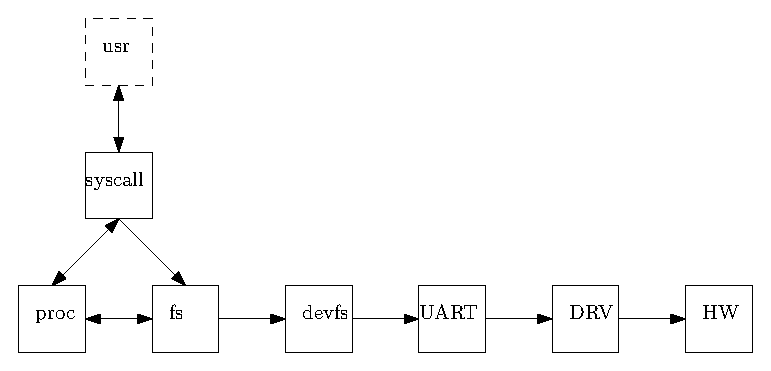
\includegraphics[width=9cm]{pics/uart}
  \caption{Communication between subsystems when a user process is writing to a UART.}
  \label{figure:dir}
\end{figure}

